\chapter{Zusammenfassung und Ausblick}\label{ch:conclusion}


\section{Figures, Zitate, Mathe}
\begin{figure}[h]
\centering
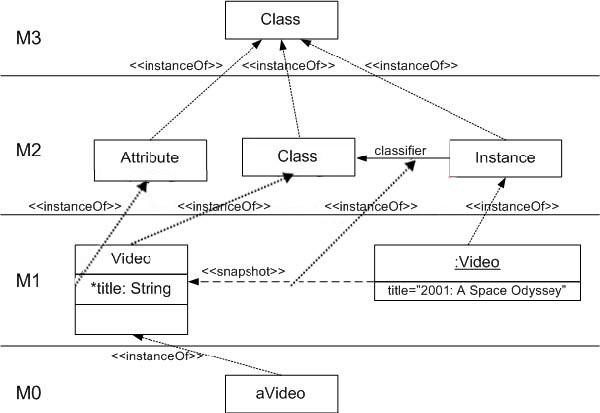
\includegraphics[scale=0.8]{OMG_MOF_4levels}
\caption{Das ist eine schlechte Grafik --- zu viele Pixel. Versuche Vektorgrafiken zu nutzen. Selbst malen geht gut mit draw.io powerpoint
  oder inkscape}\label{fig:mof}
\end{figure}

Wenn eine Abbildung verwendet wird, muss diese immer unbedingt im Text referenziert und beschrieben werden.
Z.B. so: \Cref{fig:mof}.

Zitieren geht so~\cite{haddadin2013towards}.

Math:

$A = \{x | x \in Y\}$

\begin{defs}\label{def:abc}
    A \textbf{Petrinet} is a tuple ${\Sigma = (P, T, F, W)}$.
\end{defs}

Petrinets are defined in~\Cref{def:abc}. See at the head of this document how to create your own definitions/lemma environments.


\subsection{Installation}
\textbf{Windows:} miktex

\textbf{Linux:} texlive-full

\textbf{GUI-Editor} texstudio

Konfiguration vom Editor: Preferences > Build
* default compiler: \emph{latexmk}


\section{Was ist ABC?}

\blindtext

\blindtext

\todo[inline]{Write some more}

\begin{lstlisting}[language=AST,label={lst:example-ast},caption={Example AST}]
RailwayContainer ::= Route* Region*;
abstract RailwayElement ::= <Id:int>;
Region : RailwayElement ::= TrackElement* Sensor*;
Semaphore : RailwayElement ::= <Signal:Signal>;
Route : RailwayElement ::= <Active:boolean> SwitchPosition*;
SwitchPosition : RailwayElement ::= <Position:Position>;
Sensor : RailwayElement;
abstract TrackElement:RailwayElement;
Segment : TrackElement ::= <Length:int> Semaphore*;
Switch : TrackElement ::= <CurrentPosition:Position>;
\end{lstlisting}
%
Das Listing~\ref{lst:example-ast} zeigt eine beispielhafte Grammatik, welche im Attribute im folgenden Listing genutzt wird:

\lstinputlisting[language=JRAG,style=unboxed]{code/requiredSensor.jrag}
